\documentclass[12px]{article}
\setlength{\parindent}{4em}
\usepackage[margin=2cm]{geometry}
\usepackage{graphicx}
\usepackage{amsmath}
\usepackage{amssymb}
\usepackage{enumerate}
\usepackage{multicol}
\usepackage{color}
\usepackage[font=small,labelfont=bf]{caption}
\usepackage{pifont}
\usepackage{float}
\linespread{1.5}

\begin{document}
\begin{center}
    \Large\textbf{Section 10.3, 10.4 Calculus in Polar Coordinates}
\end{center}
\begin{enumerate}
    \item Polar Coordinates
    \begin{enumerate}[(1)]
        \item Realationship between 
        Cartesian and Polar Coordinates.
        \begin{center}
            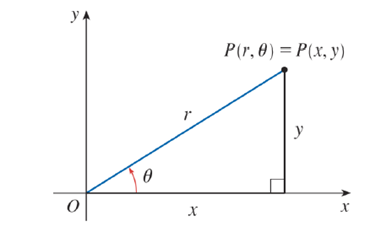
\includegraphics[width=5cm]{PolarCoordinates.png}
        \end{center}
        $$x=rcos\theta,\ y=rsin\theta,\ r^2=x^2+y^2$$
        \item Polar Curves
        \begin{enumerate}[A.]
            \item Circle\\
            $r=2asin\theta\ or\ r=2acos\theta$\\
            \\
            \\
            \\
            \\
            \item Coardiod\\
            $r=a(1\pm sin\theta)\ or\ r=a(1\pm cos\theta)$\\
            \\
            \\
            \\
            \\
            \item N-leaved Rose
            $r=acos(n\theta)\ or\ r=asin(n\theta)$\\
            \\
            \\
            \\
            \\
        \end{enumerate}
    \end{enumerate}
    \item Calculus in Polar Coordinates\\
    For a curve described in polar coordinates, $r=f(\theta)$, we know that it’s parametric equation can be described as:
    $$x=rcos\theta=f(\theta)cos\theta\text{ and }y=rsin\theta=f(\theta)sin\theta$$
\newpage
    Then, the slope can be determined by:
    $$m=\frac{dy}{dx}=\frac{dy/d\theta}{dx/d\theta}=\frac{f'(\theta)sin\theta+f(\theta)cos\theta}{f'(\theta)cos\theta-f(\theta)sin\theta}$$
    \begin{enumerate}[(1)]
        \item Categories of tangents
        \begin{enumerate}[A.]
            \item Horizontal tangents:$\frac{dy}{d\theta}=0,\ \frac{dx}{d\theta}\neq0$
            \item Vertical tangents:$\frac{dx}{d\theta}=0,\ \frac{dy}{d\theta}\neq0$
            \item Tangent line at pole: $m=tan\theta$
        \end{enumerate}
        \item Area
        $$A=\int_a^b\frac{1}{2}[f(\theta)]^2d\theta=\int_a^b\frac{1}{2}r^2d\theta$$
        \item Arc Length
        $$L=\int_a^b\sqrt{r^2+(\frac{dr}{d\theta})^2}$$
        \item Surface Area
        \begin{enumerate}[A.]
            \item Rotate about the polar axis: $S=\int_a^b2\pi(rsin\theta)\sqrt{r^2+(\frac{dr}{d\theta})^2}$
            \item Rotate about the line $\theta=\frac{\pi}{2}$: $S=\int_a^b2\pi(rcos\theta)\sqrt{r^2+(\frac{dr}{d\theta})^2}$
        \end{enumerate}
    \end{enumerate}
\end{enumerate}\leavevmode\newline
\begin{multicols}{2}
    \noindent\textbf{\textit{Example 1}}\\
    Find the points on the curve $r=1+cos\theta$ where the tangent line is horizontal or vertical.\\
    \\
    \\
    \\
    \\
    \\
    \\
    \textbf{\textit{Example 2}}\\
    Sketch the curve $r=2+2cos\theta$ and find the area that it encloses.\\
    \\
    \\
    \\
    \\
    \textbf{\textit{Example 3}}\\
    Find the exact length of the polar curve $r=\theta^2$, $0\leq\theta\leq 2\pi$\\
    \\
    \\
    \\
    \\
    \\
    \\
    \\
    \\
    \\
    \\
    \\
\end{multicols}
\end{document}